\documentclass[10pt,twocolumn,letterpaper]{article}

\usepackage{cvpr}
\usepackage{times}
\usepackage{epsfig}
\usepackage{graphicx}
\usepackage{amsmath}
\usepackage{amssymb}
%%%%%%%%%%% CVPR template packages end %%%%%%%%%%%%%%
\usepackage{verbatim} % for comment environment
% \usepackage{soul} % for \hl highlighting
% Include other packages here, before hyperref.

% If you comment hyperref and then uncomment it, you should delete
% egpaper.aux before re-running latex.  (Or just hit 'q' on the first latex
% run, let it finish, and you should be clear).
\usepackage[pagebackref=true,breaklinks=true,letterpaper=true,colorlinks,bookmarks=false]{hyperref}

%\cvprfinalcopy % *** Uncomment this line for the final submission

\def\cvprPaperID{489} % *** Enter the CVPR Paper ID here
\def\httilde{\mbox{\tt\raisebox{-.5ex}{\symbol{126}}}}

\DeclareMathOperator{\diag}{diag}

% 3D pose of the cars and ego motion
\newcommand{\uv}[1]{\hat{\mathbf{#1}}}
\newcommand{\pos}[2]{\mathbf{p}^{(#1)}(#2)}
\newcommand{\ori}[2]{\mathbf{\omega}^{(#1)}(#2)}
\newcommand{\state}[2]{\mathbf{s}^{#1}(#2)}

% ego pose
\newcommand{\egop}[1][t]{\pos{c}{#1}}
\newcommand{\egoo}[1][t]{\ori{c}{#1}}
\newcommand{\egos}[1][t]{\state{c}{#1}}

% relative pose between camera and car $i$
\newcommand{\relp}[2]{\Omega^{#1}(#2)}
\newcommand{\relpz}[2]{\Omega_z^{#1}(#2)}

% 3D tracks on car $i$ in its own coordinate frame
\newcommand{\tracklets}{\mathbf{X}^{(i)}_o}
\newcommand{\tracklet}[1]{\mathbf{x}^{(i)}_{#1}}
% track projections on camera
\newcommand{\trackp}[1]{\mathbf{u}^{(i)}(#1)}
\newcommand{\trackpj}[1]{\mathbf{u}_j(#1)}
% Unclassified track point projected on camera
\newcommand{\ucTrackp}{\mathbf{u}(t)}


% dimensions of car $i$
\newcommand{\dimsn}[1]{\mathbf{B}^{#1}}
\newcommand{\expDimsn}{\hat{\mathbf{B}}}

% projection function
\newcommand{\projectionOf}[1]{\pi_{\relp{i}{t}}\left(#1\right)}
\newcommand{\projectionOft}[1]{\pi_{\relp{i}{t+1}}\left(#1\right)}
\newcommand{\centerProj}{\bar{\pi}_{\relp{i}{t}}(\dimsn{i})}
\newcommand{\cornerProj}[1]{\pi^{#1}_{\relp{i}{t}}(\dimsn{i})}
\newcommand{\triangleProj}[1]{\triangle^{#1}_{\relp{i}{t}}(\dimsn{i})}

% bounding box corners on image
\newcommand{\bb}[1]{\mathbf{d}^{#1}(t)}

\newcommand{\Energy}[1]{\mathcal{E}^{it}_{\text{#1}}}
\newcommand{\pEnergy}[1]{\mathcal{E}^{ijt}_{\text{#1}}}
% Weighted energy
\newcommand{\WEnergy}[1]{\lambda_{\text{#1}}\Energy{#1}}
\newcommand{\EnergyCol}{\mathcal{E}^{ijt}_{\text{col}}}
\newcommand{\WEnergyCol}{\lambda_{\text{col}}\EnergyCol}

\newcommand{\occFreeProj}[1]{\Pi_{\relp{i}{t}}(#1)}
\newcommand{\minx}{x_{\text{min}}}
\newcommand{\miny}{y_{\text{min}}}
\newcommand{\maxx}{x_{\text{max}}}
\newcommand{\maxy}{y_{\text{max}}}
\newcommand{\frontface}{F^i_\text{FF}(t)}

\newcommand{\occ}[1]{o({#1})}
\newcommand{\face}{F^i_k(t)}

\newcommand{\invProjectionOf}[1]{\pi^{-1}_{\relp{i}{t}}\left(#1\right)}
\newcommand{\occf}{f^i_{occ}(\mathbf{x}_j)}
\newcommand{\occftot}{f_{occ}(\mathbf{x}_j)}
\newcommand{\occft}[1]{f_{occ}(#1)}

\newcommand{\ray}{\hat{\mathbf{r}}_j}
\newcommand{\occfray}{f_{occ}(\lambda\ray)}
\newcommand{\lambdadist}{f_{\lambda}(\trackpj{t-1}, \lambda)}

\newcommand{\occfxi}{L(\mathbf{x}; \pos{i}{t-1}, \Sigma_i)}
\newcommand{\occfi}{L(\lambda \ray; \pos{i}{t-1}, \Sigma_i)}
\newcommand{\assocP}{a^{(ij)}(\lambda)}
\newcommand{\assocPk}{a^{(ij)}(\lambda_k)}

\newcommand{\Ereproj}{E^{(ij)}_{\text{reproj}}}
\newcommand{\Ptrans}{P^{(j)}_{\text{transmission}}(\lambda)}
\newcommand{\Ptransmud}{P^{(j)}_{\text{transmission}}(\mu^{(i)}_d)}
\newcommand{\Prefl}{P^{(ij)}_{\text{reflection}}(\lambda)}
\newcommand{\dishort}{d_i(\mathbf{x})}

\newcommand{\Lu}{L_u(\mathbf{u}, \mu^i_u,\Sigma^i_u)}
\newcommand{\Llambda}{L_{\lambda}(\mathbf{u}, \lambda; \mu^i_d)}

\newcommand{\Gauss}{\mathcal{N}}
\newcommand{\PropDist}{\mathcal{W}_j}

\newcommand{\muijl}{\mu^{(ij)}_{\lambda}}
\newcommand{\sigmaijl}{\sigma^{ij}_{\lambda}}

\newcommand{\Sigmait}{\Sigma^{(i)^{-1}}_t}

\newcommand{\muit}{\mu^(i)_t}
\newcommand{\Sigmaic}{\Sigma'^{(i)^{-1}}_c}

\newcommand{\muic}{{\mu^(i)_c}}
\newcommand{\Sigmaicf}{\Sigma^{(i)^{-1}}_c}

\newcommand{\muiu}{\mu^{(i)}_t}
\newcommand{\Sigmaiu}{\Sigma^{(i)^{-1}}_u}

\newcommand{\xt}{\mathbf{x}_t}
\newcommand{\xc}{\mathbf{x}_c}

\newcommand{\Rctot}{R}
\newcommand{\tctot}{t}

\newcommand{\tcmut}{t'}


\newcommand{\Beizer}{B\'eizer }

\newcommand{\LaneUncertainty}[1]{\Sigma_{L_m}(#1)}
\newcommand{\projOnLane}[1]{\pi_{L_m(k)}(#1)}

\newcommand{\xymin}[1]{#1_{\text{min}}}
\newcommand{\xymax}[1]{#1_{\text{max}}}
\newcommand{\xmin}{\xymin{x}}
\newcommand{\xmax}{\xymax{x}}
\newcommand{\ymin}{\xymin{y}}
\newcommand{\ymax}{\xymax{y}}
\newcommand{\Tr}[3]{{}^{#1}{#2}_{#3}}

% Pages are numbered in submission mode, and unnumbered in camera-ready
%\ifcvprfinal\pagestyle{empty}\fi
%\setcounter{page}{4321}
%\DeclareMathSymbol{\Tangent}
\DeclareMathOperator{\sech}{sech}
\DeclareMathOperator{\poly}{poly}
\DeclareMathOperator*{\argmin}{\arg\min}

\begin{document}
%\title{Continuous Models for Scene and Traffic Participant Interactions in Road Scene Understanding.}
\title{Fitting convex polyhedra to project 2D bounding box}
\author{Vikas Dhiman\\
  University of Michigan\\
  Ann Arbor, MI, USA\\
{\tt\small dhiman@umich.edu}
\and
Manmohan Chandraker\\
NEC Laboratories America, Inc.\\
Cupertino, CA, USA\\
{\tt\small manu@nec-labs.com}
\and
Jason J Corso\\
  University of Michigan\\
  Ann Arbor, MI, USA\\
{\tt\small jjcorso@eecs.umich.edu}
}
\maketitle
\section{Supplementary Material}
\section{Analytic initialization}
Problem: given detection bounding box and ground plane estimate the unknown parameters i.e. position, orientation and size of the car. This problem is under-determined. Given the bounding box, we just have four constraints while we have six unknowns. To reduce the number of unknowns we assume that detection also gives us an estimate of angle and we assume that length of car is 1.3 times the height. Now, we have 4 unknowns and 4 constraints and we can solve them analytically.

\subsection{Necessary transforms}
Let the ground plane be known with parameters $(\uv{n}, h)$. Let us take the ground plane to be the XY plane with Z axis pointing upwards and origin at the point of intersection of Y-axis with ground plane. The unit vector describing the ground plane is ambiguous by sign, we choose the sign of $\uv{n}$ such that $\hat{n}_2 > 0$, i.e. the unit vector is along the positive Y-axis of the camera based on the assumption that the camera axis are approximately aligned such that Y-axis points downwards and Z-axis to the front.

\begin{align}
  ^gR_c &= [\uv{i}, -\uv{n} \times \uv{i}, -\uv{n}]\\
  ^gt_c &= [0, 0, h]^\top\\
        \text{where} & \\
 \uv{i} &= \frac{1}{\sqrt{\hat{n}^2_3, \hat{n}^2_2}}[0, \hat{n}_3, \hat{n}_2]^\top
\end{align}

In homogeneous coordinates, let the camera to ground transformation be
represented by $^gT_c = \begin{bmatrix}^gR_c & ^gt_c\\ \mathbf{0} &
1\end{bmatrix}$ and its inverse be represented by $^cT_g = {}^gT_c^{-1}$. Let
the yaw of car be given as theta in camera coordinates. Assume it to be same as
ground plane coordinates.

\begin{align}
  \Tr{g}{R}{t} &= \begin{bmatrix}
  \cos(\theta) & \sin(\theta) & 0 \\
 -\sin(\theta) & \cos(\theta) & 0 \\
             0 & 0 & 1
  \end{bmatrix}
\end{align}

\subsection{System of equations}
Let the detected bounding box be represented by $[\xmin, \ymin, \xmax, \ymax]^T$. Let $^cT_t$ be the transformation from tracklet to camera.
\newcommand{\Cu}{C_u}
\newcommand{\Cc}{C_c}
\begin{align}
  \Cu &= \begin{bmatrix}
    0.5 & 0.5 & 0\\
    0.5 & -0.5 & 0\\
    -0.5 & -0.5 & 0\\
    -0.5 & 0.5 & 0\\
    0.5 & 0.5 & 1\\
    0.5 & -0.5 & 1\\
    -0.5 & -0.5 & 1\\
    -0.5 & 0.5 & 1
  \end{bmatrix}\\
  C_i &= \diag( C_{u\{i,:\}} ) \begin{bmatrix}3& 0\\0 & 1 \\1 & 0\end{bmatrix} 
\end{align}

\newcommand{\ttg}{\Tr{g}{\mathbf{t}}{t}}
\newcommand{\tgc}{\Tr{c}{\mathbf{t}}{g}}
\newcommand{\Rgc}{\Tr{c}{R}{g}}
\newcommand{\Rtg}{\Tr{g}{R}{t}}
\newcommand{\Rtc}{\Tr{c}{R}{t}}
\newcommand{\Pgc}{\Tr{c}{P}{g}}
\newcommand{\Ptc}{\Tr{c}{P}{t}}

Consider the projection of i\textsuperscript{th} corner of the car.
\begin{align}
  \lambda_i \mathbf{u}_i &= K(\Rgc(\Rtg C_i[h, w]^\top + \ttg) + \tgc) & \text{ or }\\
  \lambda_i \mathbf{u}_i &= K\Rtc C_i [h, w]^\top + K\Rgc \ttg + K \tgc
  \label{eq:vectorproj}
\end{align}
where $\Rtc = \Rgc\Rtg$, $\ttg = [t_x, t_y, 0]^\top$ is unknown car position in
ground coordinates, $h$ is unknown height, $w$ is unknown width of the car,
$\lambda$ is unknown scale factor and $\mathbf{u}_i$ is the image projection of
i\textsuperscript{th} corner of the car.

Equation \eqref{eq:vectorproj} is a set of 3 equations, the third of which allows us to eliminate $\lambda$ as it gives the $\lambda$ and as a linear combination of $t_x$, $t_y$, $h$ and $w$. Let $\Ptc = K\Rtc$ and $\Pgc = K\Rgc$.
\begin{align}
  \lambda_i \mathbf{u}_i &=  \Ptc C_i [h, w]^\top + \Pgc \ttg + K \tgc\\
  \lambda_i &= \lambda_{hi}  h + \lambda_{wi}  w + \lambda_{tx}  t_x + \lambda_{ty} * t_y + \lambda_c\\
  \text{where} & \\
  \lambda_{hi} &= \Ptc(3, :) C_i(:, 1)\\
  \lambda_{wi} &= \Ptc(3, :) C_i(:, 2)\\
  \lambda_{tx} &= \Pgc(3, 1)\\
  \lambda_{ty} &= \Pgc(3, 2)\\
   \lambda_{c} &= K(3, :) \tgc
\end{align}

\subsection{Approximate solution}
Initial approximate solution can be obtained by assuming that $\ymax$ is the projection either of point 
\begin{align}
  \lambda_c \mathbf{u}_c &= \Ptc[0, 0, \frac{h}{2}]^\top + \Pgc \ttg + K\tgc
\end{align}

Assuming the height to be mean height, we can solve for approximate solution
for $\ttg$. Using this approximate solution find out the corner points that
correspond to the bounding box. Finally \eqref{eq:vectorproj} can be used for
the projected points to solve for exact $[h, w, t_x, t_y]$.

\subsection{Correspondence of bounding box limits to cuboid corners}
The $\xmin$ of bounding can be projection of either of the 8 points of the
cuboid. Once $\xmin$ is chosen the $\xmax$ can be limited to the remain 7
points hence $8 \times 7= 56$ possibilities and similarly $\ymin$ and $\ymax$
lead to 56 different possibilities. In this relatively unconstrained
configuration we have around $56 \times 56 = 3136$ possibilities, which is not
too big but with a little more analysis we can reduce the number. To this
effect we can use the aspect graph of a cuboid to understand the topological
changes by change in view points. Also out of 28 possible configurations in the
aspect graph, we can rule out the configurations that put camera below the
ground plane and directly above the observed car itself. This leaves us with 16
possible topological configurations, which include the symmetrical
configurations when the car is rotated by $180^\circ$. Considering $180^\circ$ symmetry we are only left with 8 possible topological configurations.

A more general way of finding the subset of aspect graph configuration that
need to be configured is to rewrite the bounding box inequalities, 

\begin{align}
  \lambda_i \xmax &\ge \Ptc(1, :) C_i [h, w]^\top + \Pgc(1, :) \ttg + K \tgc\\
  \label{eq:bbox-ineqst}
  \lambda_i \xmin &\le \Ptc(1, :) C_i [h, w]^\top + \Pgc(1, :) \ttg + K \tgc\\
  \lambda_i \ymax &\ge \Ptc(2, :) C_i [h, w]^\top + \Pgc(2, :) \ttg + K \tgc\\
  \lambda_i \ymin &\le \Ptc(2, :) C_i [h, w]^\top + \Pgc(2, :) \ttg + K \tgc \enspace.
  \label{eq:bbox-ineq}
\end{align}
Each of the above four equations is true for all 8 corners, hence there are 32 such inequalities.

The aspect graph boundaries also called the view events, occur when the view
point or the camera optical center crosses the faces of the cuboid object being
viewed. The camera optical center $o_t$ in tracklet coordinate frame is given by.
\begin{align}
  \mathbf{0} &= \Rgc(\Rtg o_t + \ttg) + \tgc\\
  o_t &= -\Rtg^\top \ttg -\Rtg^\top \Rgc^\top \tgc
\end{align}

The 6 faces of a cuboid are simple planes that can be written in terms of $h$
and $g$. A view event occurs whenever we have $o_t$ satisfying equations of any
one of the equations that represent the 6 faces. We have to find the number of
distinct regions that satisfy all of Eq
\eqref{eq:bbox-ineqst}-\eqref{eq:bbox-ineq}. Then for each distinct region we
need to find out the topological configuration that limits the number of
corners candidates for extrema. These can be sorted to create boundaries.


\section{Numerical integration}
Numerical integration is possible by computed by sampling. Samples need to be
generated from the association probability $\assocP$ for a given $j$. We take
proposal distribution to be a GMM with modes around probable reflection points.
The weights of all Gaussians in the mixture are proportional to the distance of
the point $j$ from projection of ellipsoid centre i.e. 
\begin{align}
  A_{ij} = \frac{1}{Z_j}\exp(-(\trackpj{t} - \mu^i_u)^\top\Sigma_u^i(\trackpj{t} - \mu^i_u))
\end{align}
where $Z_j = \sum_{i=1}^N A_{ij}$ and $\mu^i_u$ and $\Sigma_u^i$ are described in \eqref{eq:muiudef} and \eqref{eq:sigmauidef} respectively.
The range of Gaussian $G_i$
must be in the interval $[\|\relp{i}{t}\|, \|\relp{i}{t}\| -
\sqrt{3}\max(\dimsn{i})]$. Hence we take the mean as $\|\relp{i}{t}\| -
\frac{\sqrt{3}}{2}\max(\dimsn{i})$ and variance as
$\frac{1}{3}\max(\dimsn{i})^2$. The distribution from which we sample is 
\begin{align}
  \PropDist(\lambda) = \sum_i A_{ij} \Gauss(\lambda; \|\relp{i}{t}\| -
  \frac{\sqrt{3}}{2}\max(\dimsn{i}), \frac{1}{\sqrt{3}}\max(\dimsn{i}))
\end{align}
And the numerical integral with $K$ samples is computed by
\begin{align}
    \int_1^{\infty}
    \assocP
    \Ereproj(\lambda)
    d\lambda
    =
    \frac{1}{K}\sum_k \Ereproj \frac{\assocPk}{\PropDist(\lambda_k)}
\end{align}
where $\lambda_k$ is the $k$th sample drawn from $\PropDist(\lambda)$.

\section{Sigma of ellipsoid}
\label{sec:sigmacomputation}

\begin{align}
  \muit &= \begin{bmatrix}
  0& 0& \frac{h}{2}
  \end{bmatrix}^\top\\
  \Sigmait &= \begin{bmatrix}
    \frac{4}{l^2} & 0 & 0 \\
    0 & \frac{4}{w^2} & 0 \\
    0 & 0 & \frac{4}{h^2}
  \end{bmatrix}
\end{align}

In tracklet coordinates the equation of ellipsoid is 
\begin{align}
  (\xt - \muit)^\top \Sigmait (\xt - \muit) = 1
\end{align}


Moving to camera coordinates
\begin{align}
  (\Rctot \xc + \tctot - \muit)^\top \Sigmait (\Rctot \xc + \tctot - \muit) = 1
\end{align}

Let $\tcmut = \tctot - \muit$
\begin{align}
  (\Rctot \xc + \tcmut)^\top \Sigmait (\Rctot \xc + \tcmut) = 1
\end{align}
\begin{align}
  \xc^\top \Rctot^\top \Sigmait \Rctot \xc + 2 (\Rctot^\top \tcmut)^\top  \Rctot^\top\Sigmait \Rctot \xc
  + \tcmut^\top \Sigmait \tcmut = 1
\end{align}
Let $\Sigmaic = \Rctot^\top \Sigmait \Rctot$ and $\muic = - \Rctot^\top
\tcmut$
\begin{align}
  (\xc - \muic)^\top\Sigmaic(\xc - \muic) - \muic^\top\Sigmaic\muic +
  \tcmut^\top \Sigmait \tcmut = 1
\end{align}
Let $\Sigmaicf = \frac{\Sigmaic}{1 - \tcmut^\top \Sigmait \tcmut +
\muic^\top\Sigmaic\muic}$
\begin{align}
(\xc - \muic)^\top\Sigmaicf(\xc - \muic) = 1
\end{align}

Hence, we have following expression for mean and sigma of ellipsoid:
\begin{align}
  \label{eq:ellipsoidMeanSigma}
  \muic &= - \Rctot^\top \tcmut \\
  \Sigmaicf &= \frac{\Sigmaic}
{1 - \tcmut^\top \Sigmait \tcmut + \muic^\top\Sigmaic\muic}
\end{align}


\section{Projection of ellipsoid to image}
\newcommand{\mubar}{\bar{\mu}_i}
The perspective projection of an ellipsoid in general is not an ellipsoid in
general. We approximate the projection of ellipsoid by projecting a slice
through the ellipsoid. We choose the slice as the plane perpendicular to the
line joining the center of ellipsoid to the optical center of camera. Let
$\muic$ and $\Sigmaicf$ be the parameters of ellipsoid describing the ellipsoid
in camera coordinates. The any point $x$ on the plane satisfies
$x^\top\frac{\muic}{\|\muic\|} = \|\muic\|$. We introduce 
$\mubar = \frac{\muic}{\|\muic\|^2}$ for notational simplicity. Hence, we want
to project the points that satisfy both the equation of chosen plane and the 
ellipsoid i.e.
\begin{align}
  \mubar^\top x = x^\top\mubar &= 1\\ 
  (x-\muic)^\top\Sigmaicf(x-\muic) &= 1 \enspace.
\end{align}
We rewrite $\muic = \muic\mubar^\top x$, and $1 = x^\top\mubar \mubar^\top x$
\begin{align}
  (x-\muic\mubar^\top x)^\top\Sigmaicf(x-\muic\mubar^\top x) &= x^\top\mubar \mubar^\top x \enspace,
\end{align}
which is equivalent to 
\begin{align}
  x^\top\left((I-\muic\mubar^\top)^\top\Sigmaicf(I-\muic\mubar^\top) - \mubar \mubar^\top\right)x &= 0\enspace.
\end{align}

Note that if $u$ is a projection of $x$ to camera with intrinsic parameters
$K$, then $x = K^{-1}u$ where $u$ is in homgeneous coordinates. Hence the above equation can be re-written as
\newcommand{\Sproj}{\Sigma^{-1}_{\text{proj }i}}
\newcommand{\Sperpcut}{\Sigma^{-1}_{\text{perpcut }i}}
\begin{align}
  u^\top\Sproj u &= 0\enspace, 
\end{align}
where $\Sproj = K^{-\top}\Sperpcut K^{-1}$ and 
\begin{align}
  \Sperpcut = (I-\muic\mubar^\top)^\top\Sigmaicf(I-\muic\mubar^\top) - \mubar \mubar^\top \enspace.
\end{align}

\begin{comment}
  \section{Bounding box energy}
  \label{sec:totalBBoxEnergy}
  With abuse of notation we represent the four sides of hypothesized bounding
  box by $\projectionOf{\dimsn{i}}$ and detected bounding box by $\bb{i}$.
  Suppose the bounding box $i$ is occluded by bounding box $i$ then the
  bounding box energy becomes a pairwise term.

  \begin{multline}
    \pEnergy{occ}(\relp{i}{t}, \dimsn{i}, \relp{j}{t}, \dimsn{j}) = \\
    \sum_s \rho^{ijs}(t)\projectionOf{\dimsn{i}}_s - \bb{i}_s
               %\sum_{i=1}^N \sum_{t=s_i}^{e_i}
    %\sum_kp_{ik}^{\text{track}}(\projectionOf{\dimsn{i}} - \bb{k})^\top \pmb{\rho}(i,j,t)
  \end{multline}
  where $\rho^{ijs}(t)$ is the visibility fraction of the side $s$ of the
  bounding box. We need to compute visibility fraction we need to compute the
  occlusion mask which is explained in next few sections.

  \subsection{Visible faces from bounding boxes}

  \begin{figure}[h]
    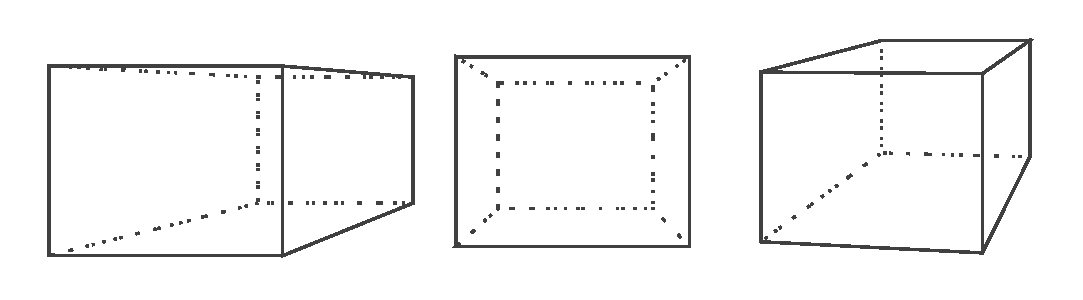
\includegraphics[width=\columnwidth]{graphics/maxFacesVisible.pdf}
    \caption{Only three faces can be visible out of six faces of a bounding
    box.}
  \end{figure}

  Each bounding box has 6 faces of which only 3 can be visible.
  Sort the vertices in increasing order of depth. The closest vertex has three
  neighboring faces. All the faces that are visible must be a subset of these
  three. Use first three vertices to
  define the front face (say $\frontface$). Also identify the four 3D points
  that correspond to min/max in x and y direction in the image. If all min-max 4
  points are same as vertices of $\frontface$, then we have only one plane
  visible. If $\{\minx, \maxx\} \not\subset \frontface \land \{\miny, \maxy\}
  \not\subset \frontface$ then we have 3 planes visible. Otherwise we have just
  two planes visible. Let number of planes visible be $n_F$.

  \begin{align}
    n_F &= \begin{cases}
    1 & \text{if }\{\minx, \maxx, \miny, \maxy\} =
    \frontface\\
    2 & \text{else if }\{x_{\text{min}}, x_{\text{max}}\} \subset \frontface \lor
    \{y_{\text{min}}, y_{\text{max}}\} \subset \frontface
    \\
    3 & \text{else if }\{x_{\text{min}}, x_{\text{max}}\} \not\subset \frontface \land
    \{y_{\text{min}}, y_{\text{max}}\} \not\subset \frontface
    \end{cases}
    \label{eq:nfaces}
  \end{align}

  First vertex restrict possible visible faces to three faces. If $n_F = 3$,
  then all three of these faces are visible. If $n_F = 2$, use second closest
  vertex to restrict visible faces to just two. If $n_F = 3$, then front face 
  $\frontface$ is the only visible face.
\end{comment}

\begin{comment}
  \subsection{Occlusion mask}
  % Initialize empty mask polygon $\occ{0}$ at depth $d=0$.
  % \begin{itemize}
  %   \item Sort all cars in increasing order of depth
  %   \item for each car $i$ in the sorted list
  %     \begin{itemize}
  %       \item Update mask polygon: \\
  %         $\occ{\relpz{i}{t}} = \occ{d} \cup \projectionOf{\dimsn{i}}$
  %       \item $d = \relpz{i}{t}$
  %     \end{itemize}
  % \end{itemize}

  % Sort all planes in increasing order of depth.  This yields a cumulative
  % occlusion mask function
  Occlusion mask is a function that takes the relative depth $d$ from the car
  camera and returns a binary mask that represents occlusions untill that depth.
  Near to the camera occlusion mask is all empty (all zeros) and more occlusions
  get added to the mask with distance.

  \begin{align}
    \occ{d} &= \begin{cases}
    \phi & \text{if } 0 < d \le \relpz{1}{t}\\
    \cup_{i=1}^j \projectionOf{F^i} & \text{if } \relpz{1}{t} < d \le \relpz{j+1}{t}
    \end{cases}
    \label{eq:occlusionmask}
  \end{align}

  where $\relpz{j}{t}$ is the depth of the $j$th TPs participant when sorted
  by increasing depth.

  \subsection{Algorithm to get faces based occlusion mask}
  \label{sec:occlusionMaskFromOptVector}

  This is an algorithm to compute occlusion mask Eq.\eqref{eq:occlusionmask}. We
  represent the occlusion mask as a set of polygons.

  Initialize empty mask polygon $\occ{0}$ at depth $d=0$.
  \begin{enumerate}
    \item Collect visible faces using Eq.\eqref{eq:nfaces} for all cars
    %\item for each face get its closest and farthest vertex to the camera.
    \item Create a sorted list of faces
    % \item Create a sorted binary tree of
    %   faces indexed by closed vertices.
    \item Loop over list of sorted visible faces
      \begin{enumerate}
        \item Get the face(s) $\{\face\}$ closer to camera than this face
        \item Add the faces to mask polygon (if not already added): \\
          $\occ{\relpz{i}{t}} = \occ{d} \cup \projectionOf{\face}$
        \item $d = \relpz{i}{t}$
      \end{enumerate}
  \end{enumerate}

  To get the occlusion mask for a face use the farthest vertex of the face to
  query $\occ{.}$.

  \subsection{Visibility fraction of a side}
  Let the center of the projected hypothesized bounding box be $\centerProj$ and
  the four corners be $\{\cornerProj{k}\}_{k=1}^{4}$ . Each side and the center
  of the bounding box form a triangle, for example $\triangleProj{1,2} =
  \{\cornerProj{1}, \cornerProj{2}, \centerProj\}$. We take the visibility of
  this triangle as a visibility of the side $s = (1,2)$. Hence the visibility
  fraction of side is given by
  \begin{align}
    \rho^{ijs}(t) = \frac{\|\triangleProj{s} \setminus \occ{\relpz{i}{t}}\|}
                         {\|\triangleProj{s}\|}
     \label{eq:bboxEnergyFromOccMask}
  \end{align}
\end{comment}

\begin{comment}
  \section{Occlusion free projection}
  Occlusion free projection can be obtained by applying the precomputed occlusion
  mask to the face projection.
  \begin{align}
    \occFreeProj{\face} &= \projectionOf{\face} \setminus
    \occ{\relpz{i}{t}}
  \end{align}

  \section{Perspective-visibility fraction}

  Apart from occlusion, we want to account for the perspective affects. When an 
  objects perspective projection is too small, detection and all related
  evidences deteriorate. One way of this is to find out the projection ratio. In
  fact, we can consolidate projection ratio and occlusion ratio in one term if
  we consider the projection of 3D bounding box planes instead of the entire
  bounding box. 

  \begin{align}
    \rho^i_t &= \sum_{k=1}^{n_F}\frac{\relpz{i}{t}^2\|\occFreeProj{F^i_k(t)}\|}{f^2\|F^i_k(t)\|}
  \end{align}

  where $\occFreeProj{.}$ again means occlusion free projection. $f$ is the
  focal length of the camera so that $\frac{f^2}{\relpz{i}{t}^2}\|F^i_k(t)\|$ is
  the area of projected plane if there were no perspective effects.
\end{comment}


\begin{comment}
  
\begin{table*}
  \begin{tabular}{|l|r|r|l|}
    \hline
    func            & equation                      & ms per 6 frames &
    comment \\
    \hline
    totalBBoxEnergy & Sec \ref{sec:totalBBoxEnergy} & 268 & \\
    laneEnergy      & Sec \ref{sec:laneEnergy}      & 163 & \\
    laneOrientationEnergy & Eq \eqref{eq:laneOrientationEnergy} & 155 & The
    equation summed up for all 6 tracklets\\
    collisionEnergyHellingerDistance & Eq 
    \eqref{eq:collisionEnergyHellingerDistance} & 93  & \\
    totalPosTransitionEnergy & Eq \eqref{eq:totalPosTransitionEnergy} & 15 & \\
    totalSizeEnergy & Eq \eqref{eq:totalSizeEnergy} & 0.9 & \\

    \hline
    occlusionMaskFromOptVector & Sec \ref{sec:occlusionMaskFromOptVector} &
    123 &
    \\
    bboxEnergyFromOccMask & Eq \eqref{eq:bboxEnergyFromOccMask} & 140 &  \\
    vis\_area\_from\_triangle & $\|\triangleProj{s} \setminus
    \occ{\relpz{i}{t}}\|$ & 76 & \\
    \hline
    distance2curve & $\text{DIST}(L_j(k), x)$ & 74 & Called 2 times per
    tracklet \\
    filterMapWaysByDistance & $M_{\text{close}} = \{m : \text{DIST}(.) < 50\} $ & 52 & \\
    area\_of\_triangle & $\|\triangleProj{s}\|$ & 48 & called 4 times per
    tracklet \\
    occlusionMask & Step 3 of Sec \ref{sec:occlusionMaskFromOptVector} & 46 &
    \\
    \hline
  \end{tabular}

  \begin{tabular}{|l|r|r|l|}
    \hline
    func            & equation                      & ms per 6 frames &
    comment \\
    \hline
    totalContPtTracksEnergy & Sec \ref{sec:totalContPtTracksEnergy} & 25000 &
    \\
    integrand & Eq \eqref{eq:integrand} & 23000 & \\
    repmat & & 5000 & \\
    assocCoeffEval & Eq \eqref{eq:assocCoeffEval} & 4000 & \\
    evalPreflection & Eq \eqref{eq:analytic-prefl} & 3000 & \\
    gradfocci & $\nabla \occf^\top \ray$ & 2040 & \\
    associationCoefficientInit & Eq
    \eqref{eq:ptransmissionInit}\eqref{eq:ellipsoidMeanSigma} & 1706 & \\
    projectToImage & $\frac{Ku}{Ku(3)}$ & 4000 & Called ~8 times per edge\\
    evalCumulativePtrans & \eqref{eq:evalCumulativePtrans} & 1178 & \\
    ptransmissionApproxInit & \eqref{eq:ptransmissionInit} & 1000 & \\
    ellipsoidCentreDist & $(x-\mu)^\top \Sigma (x-\mu)$ & 1000 & \\
    squeeze & & 951 &\\
    trackletToCamTransform & $R_{\ori{i}{t}}, t$ & 786 & \\
    ellipsoidMeanSigma & Eq \eqref{eq:ellipsoidMeanSigma} & 812 & \\
    \hline
  \end{tabular}
\end{table*}

\end{comment}

\begin{comment}%%%%%%%%%%%%% May or may not use %%%%%%%%%%%
TODO: Write Introduction
  NEC has already developed a monocular camera based structure from motion
  system which is accurate for requirements of road scene understanding. So we
  assume that egomotion is given as an observed variable in our graphical
  model. And we have following features to our disposal for estimating the 3D
  poses (position + orientation) of traffic participants (TPs):
  \begin{description}
    \item[Ground plane] We assume that all the TPs lie on a common ground
      plane. This is not particularly true for the cars that are parked off the
      road. However, for autonomous driver assistance applications we can
      ignore those cars.
    \item[Detections] We assume that 2D car detections are available with tracking informations.
    \item[Point tracks] We assume that 2D point tracks are available.
    \item[GPS and Map information] We assume that GPS information is available
      and we use openstreetmaps.org for pulling out local map for the current
      car's position.
    \item[Lane Information] We assume the lane detection works well and lane
      information is available.
    \item[Size prior] The distribution of size of cars follows gaussian distribution.
    \item[Collision] A reasonable output of the system donot has any overlapping cars.
  \end{description}
\end{comment}

  \section{Uncertainty addition in measurement}
  Consider that we have a set of measurements whose mean and variance are known $\mu = E(x)$ and $\Sigma = E ((x - \mu_x)(x - \mu_x)^\top)$. We want to know the
  affect of uncertainty on mean and variance of existing observations. On adding
  noise $[\Delta x, \Delta y]^\top$ with zero mean and covariance $\Delta
  \Sigma = E(\Delta x \Delta x^\top)$ the covariance of new data is given by
  \begin{align}
    E((x + \Delta x)(x+\Delta x)^\top) = E(xx^\top) + E(x \Delta x^\top) %\\
    + E(\Delta x x^\top) + E(\Delta x \Delta x^\top)
  \end{align}
  where the terms $E(x \Delta x^\top)$ denote the correlation between the data
  vector and the uncertainty in the data. Although we understand that in our case
  the data is the appearance based detection score and uncertainty because of
  occlusion is closely related to the appearance and hence detection score, we
  assume independence between $x$ and $\Delta x$. Hence our resultant covariance
  matrix $ E((x + \Delta x)(x+\Delta x)^\top) = \Sigma + \Delta \Sigma$
  are 4D. But that should not be a problem because the detection scores are
  modeled as $[x_{\text{min}}, y_{\text{min}}, x_{\text{max}},
  y_{\text{max}}]^\top$, we can stack the vectors in the soft occlusion region
  domain as the regions are independent of min or max variation. The parameters
  of 4D occlusion distribution are given by

  \begin{align}
    \mu'_{Oij} = [\mu_{Oij}^\top \mu_{Oij}^\top]^\top
    \Sigma'_{Oij} = \begin{bmatrix}
      \Sigma_{Oij} & \Sigma_{Oij} \\
  \Sigma_{Oij} & \Sigma_{Oij}
    \end{bmatrix}
  \end{align}

  With our
  discussion so far, the function $O_{ij}(.)$ gives an additional measure of
  uncertainty associated with each point in the space.

% Explanation of Beizer curves is not needed %%%%%%%%%%%%%%%%%%%
% A lane is modeled by four control points of a \Beizer curve $L_j = \{l_0, l_1,
% l_2, l_3\}$. The parametric curve is given by $L_j(k) = \sum_{i=0}^3 {}^3C_i
% (1-t)^{3-i}t^i l_i$. \Beizer are double differentiable so one can find
% tangents ($L'_j(k)$) and normals $R_{\frac{\pi}{2}}L'_j(k)$ where 
% $R_{\frac{\pi}{2}} = \begin{bmatrix} 0 & -1 \\ 1 & 0 \end{bmatrix}$ is
% $90^\circ$ rotation matrix.

%Using standard algorithms \cite{ma2003point, chen2007improved}, we 
%approximate the closest point on a \Beizer curve $k_x = \projOnLane{x}$.
%Consequently one can get solutions for shortest distance $s =
%\text{DIST}(L_j(k), x)$ and orientation at a closest point on the lane
%$\mathbf{t} = \text{TAN}(L_j(k), x)$.

% \subsection{Position in lane}
%
% \begin{align}
%   \Energy{plane} &=
%   \min_{j = 0}^{n_l} \text{DIST}(L_j(k), \pos{i}{t})
% \end{align}
%
 % 
 % We normalize it with the confidence in lane positions.
 % 
 % \begin{align}
 %   \Energy{plane} &=
 %   \min_{m = 0}^{n_l} \text{DIST}(L_m(k), \pos{i}{t})
 %   \LaneUncertainty{\pos{i}{t}}
 % \end{align}



%\subsection{Orientation within lane}
%\begin{itemize}
%\end{itemize}

% \begin{align}
%   \Energy{olane} &= 1 - \text{TAN}(L_l(k),  \pos{i}{t})
%   \cdot
%   \ori{i}{t}
% \end{align}
% 
% 
% 
% This model needs to be scaled by uncertainty. For example, if we want to say
% that the farther the lane is from the camera we are less sure about lane
% orientation and hence this evidence term we scale it by say square of distance
% of the car position from camera.

% \begin{align}
%   \Energy{olane} &= 
%   (1 - \ori{i}{t} \cdot \text{TAN}(L_{m^*}(k),  \pos{i}{t}) )
%   
% \end{align}
% where $m^* = \arg \min_m \text{DIST}(L_m(k), \pos{i}{t})$



\begin{comment}
    
\section{Collisions}

The collision constraint among TPs can be modelled by
pairwise distance based constraints. But having constraints between each pair
of participants is bound to create cycles and computational inefficient.
Among game developers it is common to use spatial hashing to find collision
candidates and use pairwise constraints only among those. While this will
enable us to speed up collision checking, we will still end up inducing cycles
in the model. There are two ways to break these cycles, 1) disable the cross
lane collision checking 2) created a weighted graph among collision
candidates weighted by distance and then find a minimum spanning
tree to break cycles. (1) is too strong of an assumption hence we focus on the
second approach.

There are two possible approaches to find collision among candidates (1)
polygon intersection methods (2) soft ellipse intersection method. Boost
provides scan line based approach to find intersections of polygons. Since our
polygons are simple rectangles, this approach can be very fast. Other approach
is to approximate rectangles with ellipses and finding if the ellipses
intersect.  This intersection can be computed analytically.

\begin{align}
  \EnergyCol &= \begin{cases}
  \infty &\text{if INTERSECTS}(\pos{i}{t}, \dimsn{i}, \pos{j}{t},
  \dimsn{j})\\
  0 &\text{otherwise}
  \end{cases}
\end{align}

%For smoother collision probability see Section \ref{sec:smoothercollision}.


\subsection{Ellipse-ellipse intersection}
\label{sec:ellipseintersection}
A rectangle with sides $2a$ and $2b$ can be approximated by an ellipse with
equation $\frac{x^2}{a^2} + \frac{y^2}{b^2} = 1$. But this ellipse is inside
the rectangle. To enclose the rectangle, scale the ellipse by a factor of
$\sqrt{2}$. The equation becomes, $\frac{x^2}{2a^2} + \frac{y^2}{2b^2} = 1$.
For rotation $\psi$ and center $\pos{i}{t}$, the equation of ellipse can be
re-written as:
\begin{align}
  (\mathbf{x} - \pos{i}{t})^\top\Sigma_i^{-1}(\mathbf{x} - \pos{i}{t}) &= 1
\end{align}
where
\begin{align}
  \Sigma_i^{-1} &= \begin{bmatrix}
    \frac{\cos^2{\psi}}{2a^2} + \frac{\sin^2{\psi}}{2b^2} &
    \frac{\cos{\psi}\sin{\psi}}{2}(\frac{1}{b^2} - \frac{1}{a^2})\\
    \frac{\cos{\psi}\sin{\psi}}{2}(\frac{1}{b^2} - \frac{1}{a^2}) &
    \frac{\sin^2{\psi}}{2a^2} + \frac{\cos^2{\psi}}{2b^2} \\
  \end{bmatrix}
\end{align}

% A point $\mathbf{x}$ is inside both ellipse $i$, $j$ if and only if
% \begin{multline}
%   (\mathbf{x} - \pos{i}{t})^\top\Sigma_i^{-1}(\mathbf{x} - \pos{i}{t}) +\\
% (\mathbf{x} - \pos{j}{t})^\top\Sigma_j^{-1}(\mathbf{x} - \pos{j}{t})
%   \le 2
% \end{multline}
% which is equivalent to
% \begin{multline}
%   (\mathbf{x} - \mu_c)^\top\Sigma_c^{-1}(\mathbf{x} - \mu_c)
%   + \pos{i}{t}^\top\Sigma_i^{-1}\pos{i}{t}\\
%   + \pos{j}{t}^\top\Sigma_j^{-1}\pos{j}{t}
%   - \mu_c^\top\Sigma_c^{-1}\mu_c
%   \le 2
% \end{multline}
% where $\Sigma_c = (\Sigma_i^{-1} + \Sigma_j^{-1})^{-1}$ and $\mu_c =
% \Sigma_c(\Sigma_i^{-1}\pos{i}{t} + \Sigma_j^{-1}\pos{j}{t})$.
% 
% There is at least one point inside both ellipse if 
% \begin{align}
%   \pos{i}{t}^\top\Sigma_i^{-1}\pos{i}{t}
%   + \pos{j}{t}^\top\Sigma_j^{-1}\pos{j}{t}
%   - \mu_c^\top\Sigma_c^{-1}\mu_c
%   &\le 2
% \end{align}
% 
% The left hand side can be interpreted as distance between two ellipses, which
% is 2 when the two ellipses collide and $0$ when two ellipse completely
% overlap.

\subsection{Smoother collision probability}
\label{sec:smoothercollision}
%The above mentioned ellipse-ellipse intersection formulation gives us an
%insight: the distance between two oriented ellipse boundaries can be again
%formulated as a distance metric\footnote{TODO:proof}.
Instead of using Gaussians to model
collision constraints as done by \cite{milan2013continuous}, we use a more
steeper sigmoid function.
\begin{multline}
  \EnergyCol = \frac{1}{1 +
\exp(-k(\pos{i}{t}^\top\Sigma_i^{-1}\pos{i}{t})-1)}\\
\frac{1}{1 +
\exp(-k(\pos{j}{t}^\top\Sigma_j^{-1}\pos{j}{t})-1)}
\end{multline}
where $k$ is steepness parameter.
%$d(.)$ is the distance metric defined as:
%\begin{multline}
%  d(\pos{i}{t}, \dimsn{i}, \pos{j}{t}, \dimsn{j})
%  =
%  \pos{i}{t}^\top\Sigma_i^{-1}\pos{i}{t} \\
%  + \pos{j}{t}^\top\Sigma_j^{-1}\pos{j}{t}
%  - \mu_c^\top\Sigma_c^{-1}\mu_c
%\end{multline}

\end{comment}



\begin{comment}
\section{Analytical attempt to integration}
  %%%%%%%%%%%%%%%% Analytical attempt to integration %%%%%%%%%%%%%%%%%%%%%
  \begin{align}
    E^i_{\text{reproj}}(\lambda) &= \left\|\trackpj{t} - \frac{p_{1:2}\lambda +
  q_{1:2}}{p_3\lambda + q_3}\right\|^2\\
  &= \frac{(p_1\lambda + q_1 - u_{j1}(t))^2 + (p_2\lambda + q_2 - u_{j2}(t))^2}
  {(p_3\lambda + q_3)^2}\\
  &= \frac{a\lambda^2 + b\lambda + c}{(p_3\lambda + q_3)^2}
  \end{align}
  where $a = p_1^2 + p_2^2$, $b = 2p_1(q_1 - u_{j1}(t)) + 2p_2(q_2 - u_{j2}(t))$
  and $c = (q_1 - u_{j1}(t))^2 + (q_2 - u_{j2}(t))^2$

  So, in terms of $\lambda$ we have the integrand as
  \begin{multline}
    \int_1^\infty
    \prod_i (1 +
    \tanh(\poly^{(1)}_{ij1}(\lambda)))\sech^4(\poly^{(2)}_{ij2}(\lambda))\\
    (\max\{ 0, \poly^{(2)}_{ij3}(\lambda) \})^2
    \frac{\poly^{(2)}_{ij4}(\lambda)}{(\poly^{(1)}_{ij5}(\lambda))^2}d\lambda
  \end{multline}
  where $\poly^{(n)}_{ijk}$ denotes a polynomial $k$ of order $n$ dependent upon $i$th
  TP and $j$th point. This integrand is still too difficult to
  be solved or approximated analytically.

  We approximate the expression,

  \begin{multline}
    \prod_i \Llambda
  \sech^4\left(\frac{k}{2}\dishort\right)(\max\{ 0, \nabla k\dishort^\top\ray \})^2
  \end{multline}

  with a
  gaussian with mean at $\mu^{ij}_{\lambda} : d_i(\mu^{ij}_{\lambda}\ray) = 0$
  standard deviation as $\sigma^{ij}_{\lambda} =
  \frac{\pi}{2\sqrt{3}kd(\mu^{ij}_{\lambda}\ray, \pos{i}{t-1})}$  and magnitude as the
  expression computed at mean. An integrand of the form
  \begin{align}
    \frac{\poly^{(2)}_{ij4}(\lambda)}{(\poly^{(1)}_{ij5})^2}
      e^{\frac{- (\lambda -
  \mu^{ij}_{\lambda})^2}{\sigma^{ij}_{\lambda}}}
  \end{align}
   is integrable analytically by parts.

   \begin{align}
   \int_1^\infty \frac{a\lambda^2 + b\lambda + c}{(p_3\lambda + q_3)^2}e^{\frac{- (\lambda -
  \mu^{ij}_{\lambda})^2}{\sigma^{ij}_{\lambda}}}d\lambda
   \end{align}
   Substituting $y = \frac{\lambda - \mu^{ij}_{\lambda}}{\sigma^{ij}_{\lambda}}$

   \begin{align}
     \int_1^\infty \frac{a_y y^2 + b_yy + c_y}
     {(p_{3y}y + q_{3y})^2}e^{-y^2}dy
   \end{align}
   where $a_y = a(\sigmaijl)^3$, $b_y = (2a\muijl + b)(\sigmaijl)^2$ and $c_y =
   (2a(\muijl)^2 + b\muijl + c)\sigmaijl$ and $p_{3y} = \sigmaijl p_3$ and
   $q_{3y} = p_3\muijl + q_3$
  
\end{comment}


  % \subsection{Sandwich of ellipsoids model}
  % 
  % \begin{enumerate}
  %   \item Model $\occf$ as
  %     sigmoid over ellipse instead of a gaussian.
  %     \begin{align}
  %       \occf = \frac{1}{
  %       1 + e^{-(\mathbf{x} - \pos{i}{t})^\top
  %         \Sigma_i (\mathbf{x} - \pos{i}{t}))}}
  %     \end{align}
  %   \item To get the intuition of this occupancy function imagine the traffic
  %     participant as layered ellipsoid. The innermost ellipsoid has very high
  %     probability (approx 1) of being occupied. The outermost ellipsoid has very
  %     low probability (approx 0) of being occupied. We will just consider the
  %     occupancy interplay within these two ellipsoids.
  %   \item Project outer ellipsoids of all TP's on the image.
  %   \item Consider the ellipses that bound the track point $\trackpj{t-1}$.
  %   \item For each ellipse do
  %     \begin{itemize}
  %       \item Case 1: The ray intersects inner ellipse
  %         Now the ray intersects both inner and outer ellipse
  %         Compute the intersection points on both the ellipses
  %         Compute the gradient function $\nabla\occf^\top \ray$ at
  %         the mid point of the two intersections. Use this as the magnitude of
  %         gaussian mixture component centered at the mid point of intersections
  %         and spread such that 97 percentile of probability mass of guassian is
  %         within the intersection points. With the same parameters model the
  %         transimission probability with product of logistic function $L(.)$.
  %       \item Case 2: The ray do not intersects inner ellipse.
  %         The ray just passes through the outer ellipse. Find the point on the
  %         ray closest to the center of the ellipse. Compute gradient function
  %         at the closest point, which will be again used as the magnitude of
  %         gaussian mixture component centered at the closest point and spread
  %         such that 97 percentile of probabiltiy mass of gaussian is within the
  %         two intersection points of the ellipse. With the same parameters model
  %         the transimission probability with product of sigmoids.
  %     \end{itemize}
  %   \item Now this approximated $\lambdadist = \sum N(.) \prod (1 - L(.))$ can
  %     be used in integrating the error over $\lambda$.
  % \end{enumerate}
  \newpage

  \clearpage
  %%%%%%%%%%%%%%%% Analytical attempt to integration %%%%%%%%%%%%%%%%%%%%%

% \section{Object detection score}
% \begin{align}
% \Energy{det}(\relp{i}{t}, \dimsn{i}) = 
%              \frac{1}{S_t^2(\projectionOf{\dimsn{i}})}
% \end{align}

% \section{Object 2D bounding box with occlusion}
% Reproduced from \cite{song2014eccv} section 4.3
% 
% \begin{multline}
%   \Energy{box}(\relp{i}{t}, \dimsn{i}) =
%              %\sum_{i=1}^N \sum_{t=s_i}^{e_i}
%              \rho^i_t \|\projectionOf{\dimsn{i}} -
%              \bb{i}\|^2
% \end{multline}
% 
% where $S_t(.)$ is the function to approximate the detection scores using
% mixture of Gaussian model and $\rho^i_t$ is the visibility fraction. 
% 
% % It can be
% % computed by using polygon intersection algorithms.
% % \begin{align}
% %   v^i_t &= \frac{\|\occFreeProj{\dimsn{i}}\|}
% %                 {\|\projectionOf{\dimsn{i}}\|}
% % \end{align}
% % where $\|.\|$ represents the norm or the area of the polygon.
% 
% Another approach is to just consider the corner points in the occlusion free
% area.  Say $\projectionOf{\dimsn{i}} = [b^i_1, \dots, b^i_4]$.
% \begin{multline}
%   \Energy{box}(\relp{i}{t}, \dimsn{i}) =
%              %\sum_{i=1}^N \sum_{t=s_i}^{e_i}
%              %S_t^2(\projectionOf{\dimsn{i}})
%              \sum_{{b^i_j} \in \occFreeProj{\dimsn{i}}}
%              \|b^i_j - d^i_j\|^2
% \end{multline}
% 
% In the opinion of this author, the second approach is better because the
% visibility is an area based measure while the error metric is point to point
% distance based measure. If we use bounding overlap instead of corner to corner
% distance, the use of visibility fraction makes much more sense. However, one
% can argue that even detection score is an area based measure. 
% 
% Hence a third approach can be 
% \begin{multline}
%   \Energy{box}(\relp{i}{t}, \dimsn{i}) =
%              %\sum_{i=1}^N \sum_{t=s_i}^{e_i}
%   \rho^i_t \|\projectionOf{\dimsn{i}} \ominus \bb{i}\|
% \end{multline}
% where $A \ominus B$ represents the symmetric difference between set $A$ and set
% $B$ and is given by $A \ominus B = (A \cup B) \setminus (A \cap B)$.
% One may argue that we can take the intersection of occlusion free projection 
% and get rid of the visibility fraction, but that would be a little off the 
% detection bounding box is usually more close to the projection of full car
% instead of the just the visible portion.
% 
% 
% \section{Orientation cues}
% There are two orientation cues (1) orientation from detection (2) orientation
% from appearance map \cite{yao2012describing}.
% 
% \begin{align}
%   \Energy{ori} &= 
%   %S_t^2(\projectionOf{\dimsn{i}})
%   \rho^i_t(1 - \cos({\omega}^i_{\text{det}} - \ori{i}{t})
% \end{align}
% 
% Appearance map is a shape prior that requires \emph{Scene labeling} input.



\end{document}
